% !TEX root = ../YourName-Dissertation.tex

\chapter{Effect of IGT on Local Governments' Spending Side}
This chapter talks about the reaction of subnational governments in the interaction with central government.The most frequently investigated question is the effect of IGT, A bunch of scholars devote time and energy to analyze and evaluate the impact of intergovernmental transfers. I summarize the literature into three categories. The first category focus on the impact on local governments' spending behavior. Under the local governments' spending behavior, two directions are highly documented. First direction concentrate on the effect of intergovernmental transfer on overall spending amounts of subnational government,such as the investigation on flypaper effect. Another direction investigate the micro-segments of the local governments' spending preference. The second category talks about the impact on local governments' revenue collection behavior, such as the investigation on local governments' tax effort, debt expansion tendency and issue and soft budget constrain behavior. The third category is about the effect of intergovernmental transfer across jurisdictions, such as the role of intergovernmental transfer in equalization. This chapter gives an overview on the most innovative literature and introduced the game theory tool under asymmetric setting to generate a theoretical model. The investigation directions can be summarized as Figure \ref*{Figure 3.1}.



\begin{figure}[H]
    \centering
    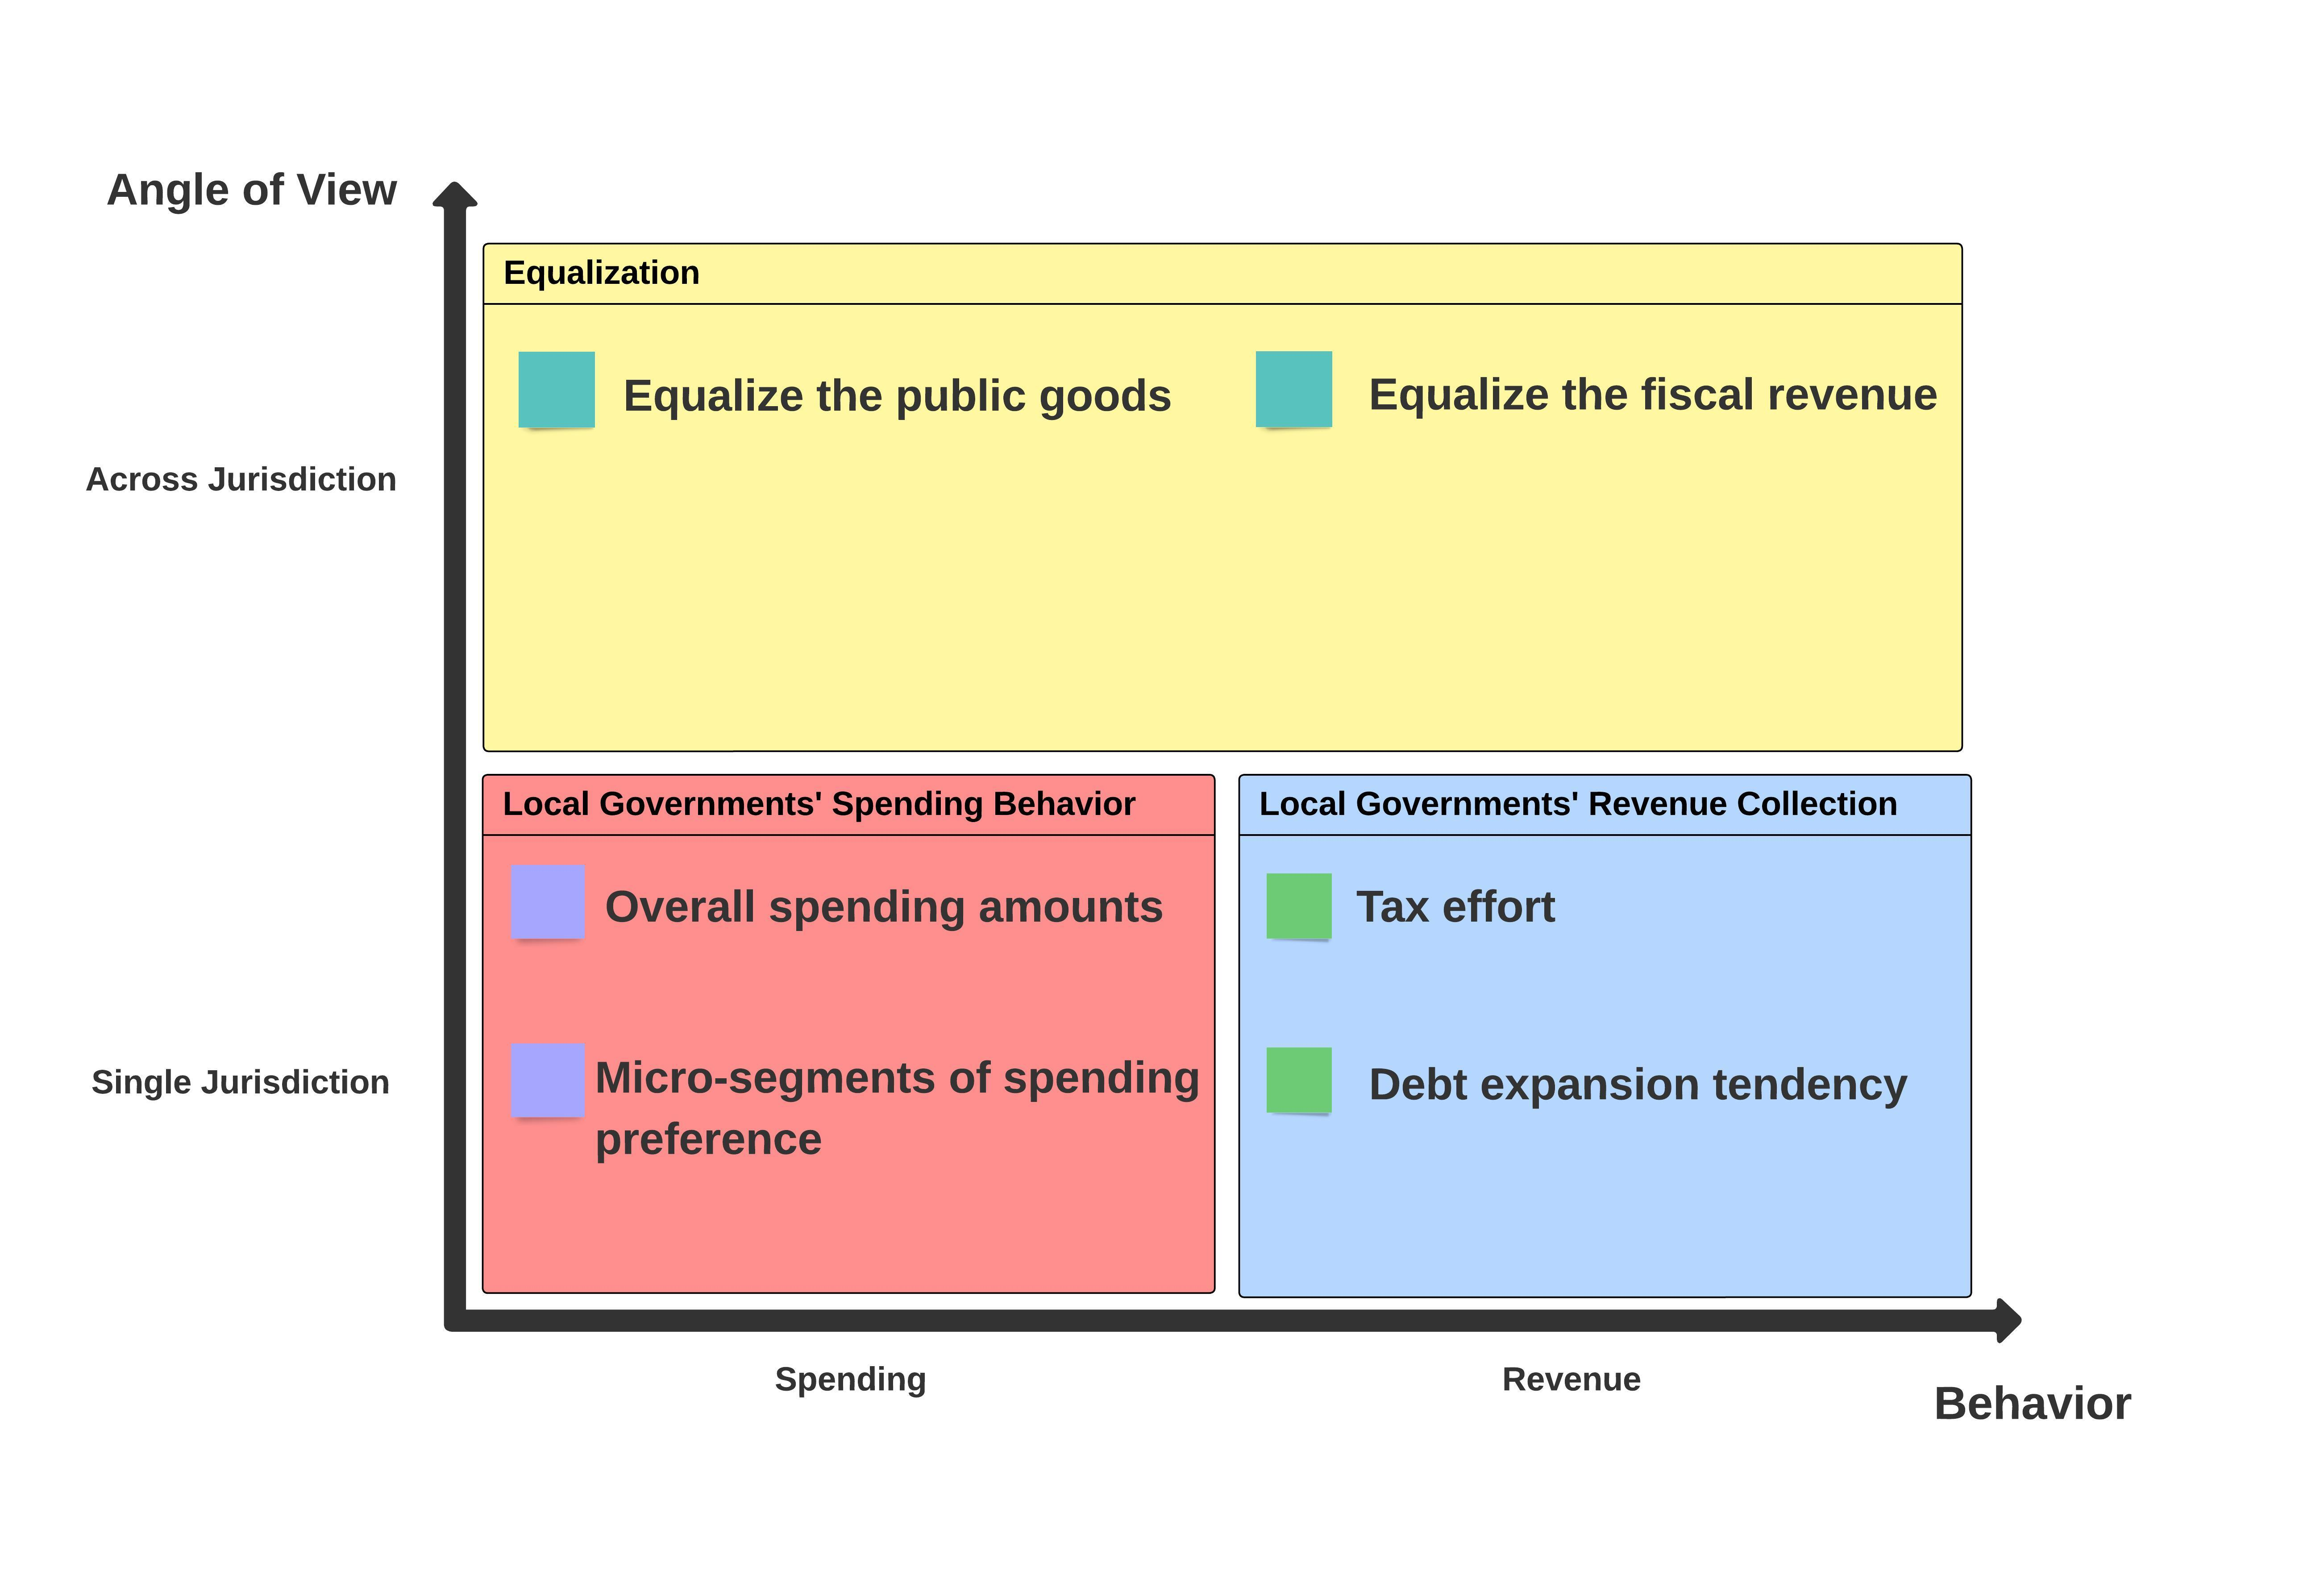
\includegraphics[scale=0.4]{Chapter-4/Figures/Effect of Intergovernmental Transfer.jpeg}
    \caption{Effect of Intergovernmental Transfer
        \texttt{} }
    \label{Figure 3.1}
\end{figure}




\section{Effect of IGT on Local Governments' Spending}

\subsection{Effect of IGT on Local Governments' Total Spending Amounts}

One intuitive philosophy is called "fungibility" \cite{pack1993foreign}, which means the intergovernmental transfer received by local government would substitute the local government's revenue. recipients assimilate dederal funds into general revenue and reduce the spending on public goods through a reduction of local taxes within the jurisdiction. However, supportive empirical evidence are quite limited. On the contrary, evidence on flypaper effect is widespread everywhere.

The flypaper effect is widely regarded as the most influential phenomenon in the fiscal federalism literature regarding the vertical transfer of funds from the federal to the state or local level \cite{hines1995anomalies,gamkhar2007impact}. According to Bradford and Oates' model, a lump sum grant to the state or local level should have the same effect as an increase in individual revenue within the jurisdiction in terms of stimulating public expenditure \cite{bradford1971analysis}. This conclusion is known as the equivalence theorem, which is based on two fundamental assumptions: the median voter theorem and lump-sum tax collection by federal, state, and local governments. However, empirical evidence does not support this theorem. Specifically, some researchers have found that a \$1 increase in individual revenue leads to an increase in public expenditure of only \$0.02 to \$0.05, while a \$1 increase in intergovernmental transfers can lead to an increase in public expenditure of \$0.25 to even \$1 \cite{bailey1998flypaper,dollery1996empirical,gamkhar2007impact}. This phenomenon is known as the flypaper effect. According to Inman's statistics, over 3,500 research papers have investigated the flypaper effect, both theoretically and empirically \cite{inman2008flypaper}.

In this section, I’m summarizing how scholars in different stages explain the flypaper effect. The understanding of flypaper effect went through a incremental progress, though may not be chronologically. This progress can be identified as three phrases. In the first stage, the conventional analysis, scholars believe the matching grants have both price effect and income effects while the non-matching grants is analogous to the lump-sum subsidy, which means only income effects exists. In second stage, some scholars start to realize that non-matching grants has price effects as well, but that’s due to the impact of fiscal federalism setting and fiscal illusion. Federal government collecting revenue then redistributing to state and local generates fiscal illusion since this process is too complicated for consumers to perceive. In third stage, scholars start to realize the effect of distortionary tax that collect by grants recipient. The distortionary tax policy together with the low administrative efficiency in state and local leads to a higher marginal cost of the tax collection. Hence no matter the grants is matching or non-matching, the state or local government trend to use the grants rather than the tax revenue to cover the expenditure.

I set up a theoretical model and introduced the asymmetric setting into the model to explain all the local governments' reactions mentioned above. Started from a very simple Ramsey model and generalize it to more complicated scenarios.

\textbf{Benchmark model}

The Benchmark model is similar to Carlos and Guillermo's \cite{vegh2016unsticking} benchmark model with small modification.

To make the benchmark model as straight forward as possible while capture the IGT mechanism. I assume that:

\begin{enumerate}
    \item Economy is static.
    \item Only one local government and representative citizen in this economy.
    \item Two kinds of goods in the economy which are public good $G$ \label{G} and private good $X$.\label{X}
    \item Resident spend all there income $y$, which is given, on either private goods $X$ or tax $\tau$.\label{y}
    \item The tax is lump-sum tax with no dissertation.
    \item Source of government revenue: tax $\tau$ and transfer $f$.\label{f}
    \item Type of transfer: Nonmatching grants,like lump-sum subsidy.
\end{enumerate}

The representative citizen's budget constraint is:
\begin{equation}
    y=X+\tau \label{bmrc budgetc}
\end{equation}
The local government's budget constraint is:
\begin{equation}
    f+\tau=G \label{bmlg budgetc}
\end{equation}
Combine equation \ref{bmrc budgetc} and \ref{bmlg budgetc}, I get a budget constraint for the economy:
\begin{equation}
    y+f=X+G \label{bmecoconstrain}
\end{equation}
The utility for representative resident comes from the utility of $X$ and $G$. I assume the utility function is the Cobb-Douglas form thus it's a concave utility:
\begin{equation}
    U(X,G)=AX^{\alpha}G^{1-\alpha} , 0<\alpha<1 \label{bmrcutility}
\end{equation}
For the representative resident, the problem is to choose proper level of $X$ to maximize the utility in equation \ref{bmrcutility} subject to equation \ref{bmrc budgetc}. The Lagrangian equation can be set up as:
\begin{equation}
    L(X)=AX^{\alpha}G^{1-\alpha}+\lambda_{rc}(y-X-\tau)  \label{bmrclagrangian}
\end{equation}
Solving the equation \ref{bmrclagrangian} will get first order condition(foc):
\begin{equation}
    \alpha A\left(\frac{X}{G}\right)^{\alpha-1}=\lambda_{r c} \label{lamdarc}
\end{equation}
\begin{equation}
    y=X+\tau \label{rcfoc}
\end{equation}
To solve the Ramsey problem, the Ramsey planner needs to decide the level of $X,G$ to maximize the utility subject to equation \ref{bmecoconstrain} and equation \ref{bmlg budgetc}. The Lagrangian can be set as:
\begin{equation}
    L(X,G)=AX^{\alpha}G^{1-\alpha}+\lambda_{e}(y+f-X-G)+\lambda_{lg}(f+\tau-G)  \label{bmeclagrangian}
\end{equation}
Solving the equation \ref{bmeclagrangian} will generate:
\begin{equation}
    \alpha A\left(\frac{X}{G}\right)^{\alpha-1}=\lambda_e+\lambda_{l g}
    \label{foc on X}
\end{equation}
\begin{equation}
    (1- \alpha) A\left(\frac{X}{G}\right)^{\alpha}=\lambda_e+\lambda_{l g} \label{foc on G}
\end{equation}
\begin{equation}
    y+f=X+G \label{foc on lambdae}
\end{equation}
\begin{equation}
    f+\tau=G \label{foc on lambdalg}
\end{equation}

Combining equation \ref{foc on X}, \ref{foc on G}, \ref{foc on lambdae} will generate:
\begin{equation}
    (1-\alpha)y+(1-\alpha)f=G \label{bmresult}
\end{equation}
The flypaper effect definition can be mathematically expressed as $\frac{d G}{d f}-\frac{d G}{d y}$. Given equation \ref{bmresult}, the flypaper effect $fe=0$, which means, under this setting, theoretically there should be no flypaper effect.
\subsubsection{Phrase One}
Except for the introduction of intergovernmental transfer in Chapter \ref*{chapter1:Introduction}, one important concern about IGT in economic analysis is the matching mechanism. For matching grants, federal governments will reimburse a specific ratio for each 1 dollar of state and local expenditure. Based on whether federal government set a cap on the matching grants, matching grants can be divided into open-ended matching grants and closed-ended grants.
%%%%%%%%%%%%%%%%%%%%%%%%%%%%%%%%%%%%%%%%%%%%%%%%%%%%%%%%%%%%%%%%%%%%%%%%%%%%%
% \textbf{Model with matching grants}

% I loosen the last assumption in the benchmark model, now the intergovernmental transfer is 100\% matching grants which is expressed as $f_m$. Suppose the matching ratio is $m$ and $0<m<1$  \label{mr}.Thus the new budget constraint for local government is:
% \begin{equation}
%     \left\{\begin{array}{l} \label{mlgbudgetc}
%         f_m+\tau=G \\
%         f_m=m G
%     \end{array}\right.
% \end{equation}
% And the budget constraint for the whole economy is:
% \begin{equation}
%     \left\{\begin{array}{l} \label{mebudgetc}
%         y+f_m=X+G \\
%         f_m=m G
%     \end{array}\right.
% \end{equation}
% Thus the Ramsey problem is to choose proper level of $X$ and $G$ to maximize the utility subject to equation \ref{mebudgetc} and equation \ref{mlgbudgetc}.
% So the new Lagrangian can be listed as:

% \begin{equation} \label{mlagrangian}
%     L(X,G)=AX^{\alpha}G^{1-\alpha}+\lambda_{e}(y+f_m-X-G)+\lambda_{lg}(f_m+\tau-G)
% \end{equation}

% Solving the equation \ref{mlagrangian}, I get foc conditions:
% \begin{equation} \label{mfocs}
%     \left\{\begin{array}{l}\alpha A X^{\alpha-1} G^{1-\alpha}=\lambda_e+\lambda_{l g}  \\  (1-\alpha) A X^\alpha G^{-\alpha}=\lambda_e+\lambda_{\lg }   \\ y+f_m=X + G \\ f_m=m G\end{array}\right.
% \end{equation}

% By letting focs in equation \ref{mfocs} equals to zero, I get following equations:
% \begin{equation} \label{myxandg}
%     G=\frac{1-\alpha}{1-m + m \alpha} y
% \end{equation}

% with $G = \frac{1}{m}$, the flypaper effect is calculated as $fe=\frac{d G}{d f_m}-\frac{d G}{d y}$
% which equals to:
% \begin{equation} \label{mfe}
%     \frac{d G}{d f_m}-\frac{d G}{d y}=\frac{2 m \alpha-2 m-\alpha+2}{m[(1-\alpha)(1-m)+1]}
% \end{equation}

% \begin{figure}[H]
%     \centering
%     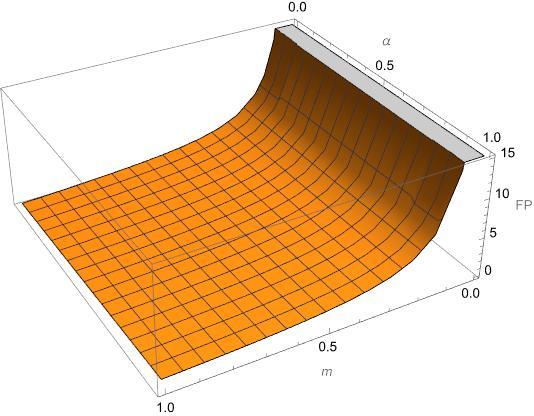
\includegraphics[scale=0.7]{Chapter-3/Figures/matchfp.jpg}
%     \caption[Flypaper Effect with Matching Grants]{Flypaper Effect with Matching Grants
%         \texttt{} }
%     \label{Figure 3.2}
% \end{figure}
% Equation \ref*{mfe} could be proved to be greater than zero, which means for matching grants, the marginal contribution on public spending is higher than the marginal contribution of private income increase.\footnote[1]{The proof process is supplied in Appendix C}
%%%%%%%%%%%%%%%%%%%%%%%%%%%%%%%%%%%%%%%%%%%%%%%%%%%%%%%%%%%%%%%%%%%%%%%%%%%

\begin{figure}[H]
    \centering
    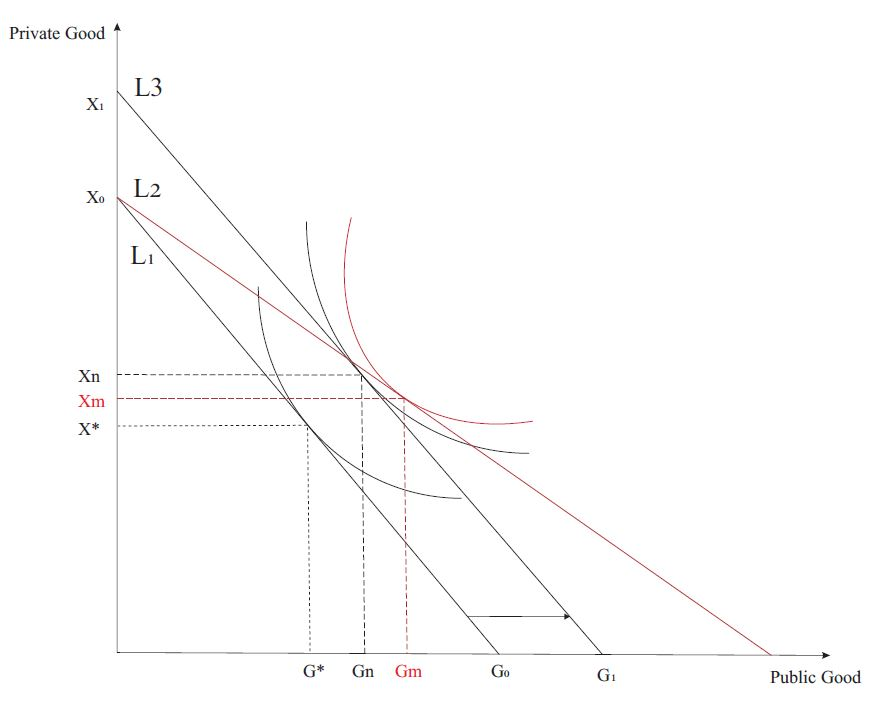
\includegraphics[scale=0.4]{Chapter-4/Figures/mfyeffect.jpg}
    \caption[Income Effect and Price Effect of Matching and Non-matching Grants]{Income Effect and Price Effect of Matching and Non-matching Grants
        \texttt{} }
    \label{Figure 3.3}
\end{figure}

As is shown in figure \ref{Figure 3.3}, the two parallel lines $L1$ and $L3$ are budget constraint of the economy before and after the non-matching grants and $L3$ is the budget constraint with matching grants which is the red line. The difference between $G_m$ and $G*$ is the combination of price effect and income effect of matching grants.

The matching grants model explains why scholars in first stage explain the fly paper effect by misspecification or omitted variable. Misspecification refers to instances where researchers may conflate matching grants with lump-sum grants, leading to a mix-up of price effects and subsequently resulting in increased public goods spending \cite{lankford1987note,henderson1968local}. Matching grants reduce the marginal price of public services, thus mix-up with lump-sum grants would lead to an increase in public goods spending \cite{gramlich1997state}. Some scholars attribute the flypaper effect to omitted variables or pre-selection issues. Knight \cite{knight2002endogenous} developed a two-level bargaining model to demonstrate that the federal government distributes intergovernmental transfers to states and local governments with a higher propensity to spend, indicating that the flypaper effect is not a result of intergovernmental transfers. However, prior studies and investigations have encountered endogeneity issues. To address this, Knight conducted an empirical test where he employed an instrumental variable to control for the endogeneity problem. His results indicate that once the pre-selection issue is filtered out, the flypaper effect is not evident, at least for the data he collected regarding interstate highway programs. To summarize, the understanding under this view is that the flypaper effect may not actually exist, but may instead be a result of misspecification or omitted variables.

\subsubsection{Phrase two}
The literature on the flypaper effect has also been approached from a second perspective, whereby scholars recognize the importance of lump-sum grants and their potential price effects. While scholars in the first stage focused on the price effects of matching grants, it was realized that this may not be sufficient to explain the large gap in the flypaper effect. As such, the second stage of literature argues that non-matching grants also have price effects, which can be attributed to fiscal illusions. McCulloch \cite{mcculloch1845treatise} argued that taxpayers often misperceive the costs of governmental activities, a concept later summarized as fiscal illusions. The theory of fiscal illusion was first developed by Italian economist Amilcare Puviani in his 1903 book \textit{Teoria della illusione finanziaria} \cite{puviani1903teoria}. Wagner  \cite{wagner1976revenue} introduced this concept in America and identified the effect of fiscal illusions on local government spending. Oates and Borge \cite{oates1979lump,borge1995lump} also recognized the potential price effect of non-matching grants and attempted to explain it using the concept of fiscal illusions. The lower-estimated public good price generates a even flatter slope of the budget constraint compared to the $L_3$ in figure \ref{Figure 3.3}.

The existence of fiscal illusion can be attributed to administrative factors and institutional intention. The fiscal federalism framework is complex and difficult for residents to comprehend, while administrative processes are often opaque and lack transparency, preventing residents from understanding the nuances of intergovernmental grants and their own contributions to these grants. Empirical research by Turnbull \cite{turnbull1998overspending} supports this view, demonstrating that imperfect information generates a broader fiscal illusion based on municipal data. Additionally, the budget-maximizing tendencies of bureaucratic systems are supported by both empirical evidence and theoretical inference \cite{mueller2003public,brennan1977towards}. This tendency is sometimes referred to as "Leviathan government," in which governments seek to maximize their budgets rather than prioritize residents' utility \cite{quigley1986budget}. The combination of budget-maximizing bureaucrats and lower perceived prices of public goods leads to increased expenditure on public goods.


\subsubsection{Phrase Three}

In stage three, Scholars have also examined the effect of the cost of tax collection within a jurisdiction. This cost can arise from two aspects, one being the distortionary tax, another one comes from the revenue collection ability of the sunational government. Assuming that tax revenue collection does not cause any distortion for the recipient is a strong assumption. In reality, changes in state and local government tax policies can significantly alter residents' behavior. For instance, if residents are dissatisfied with tax and public goods policies, they may choose to work less and spend more time on leisure. Alternatively, they may move to another jurisdiction, which itself incurs costs due to the tax increase.Hamilton \cite{hamilton1986flypaper} was the first to observe that the cost of tax collection within a jurisdiction leads to a curved budget constraint, rather than a straight line. However, his idea was not widely accepted at the time, and he neglected to consider administrative ability as a source of cost, focusing only on deadweight loss as the source of tax collecting cost.

\begin{figure}[H]
    \centering
    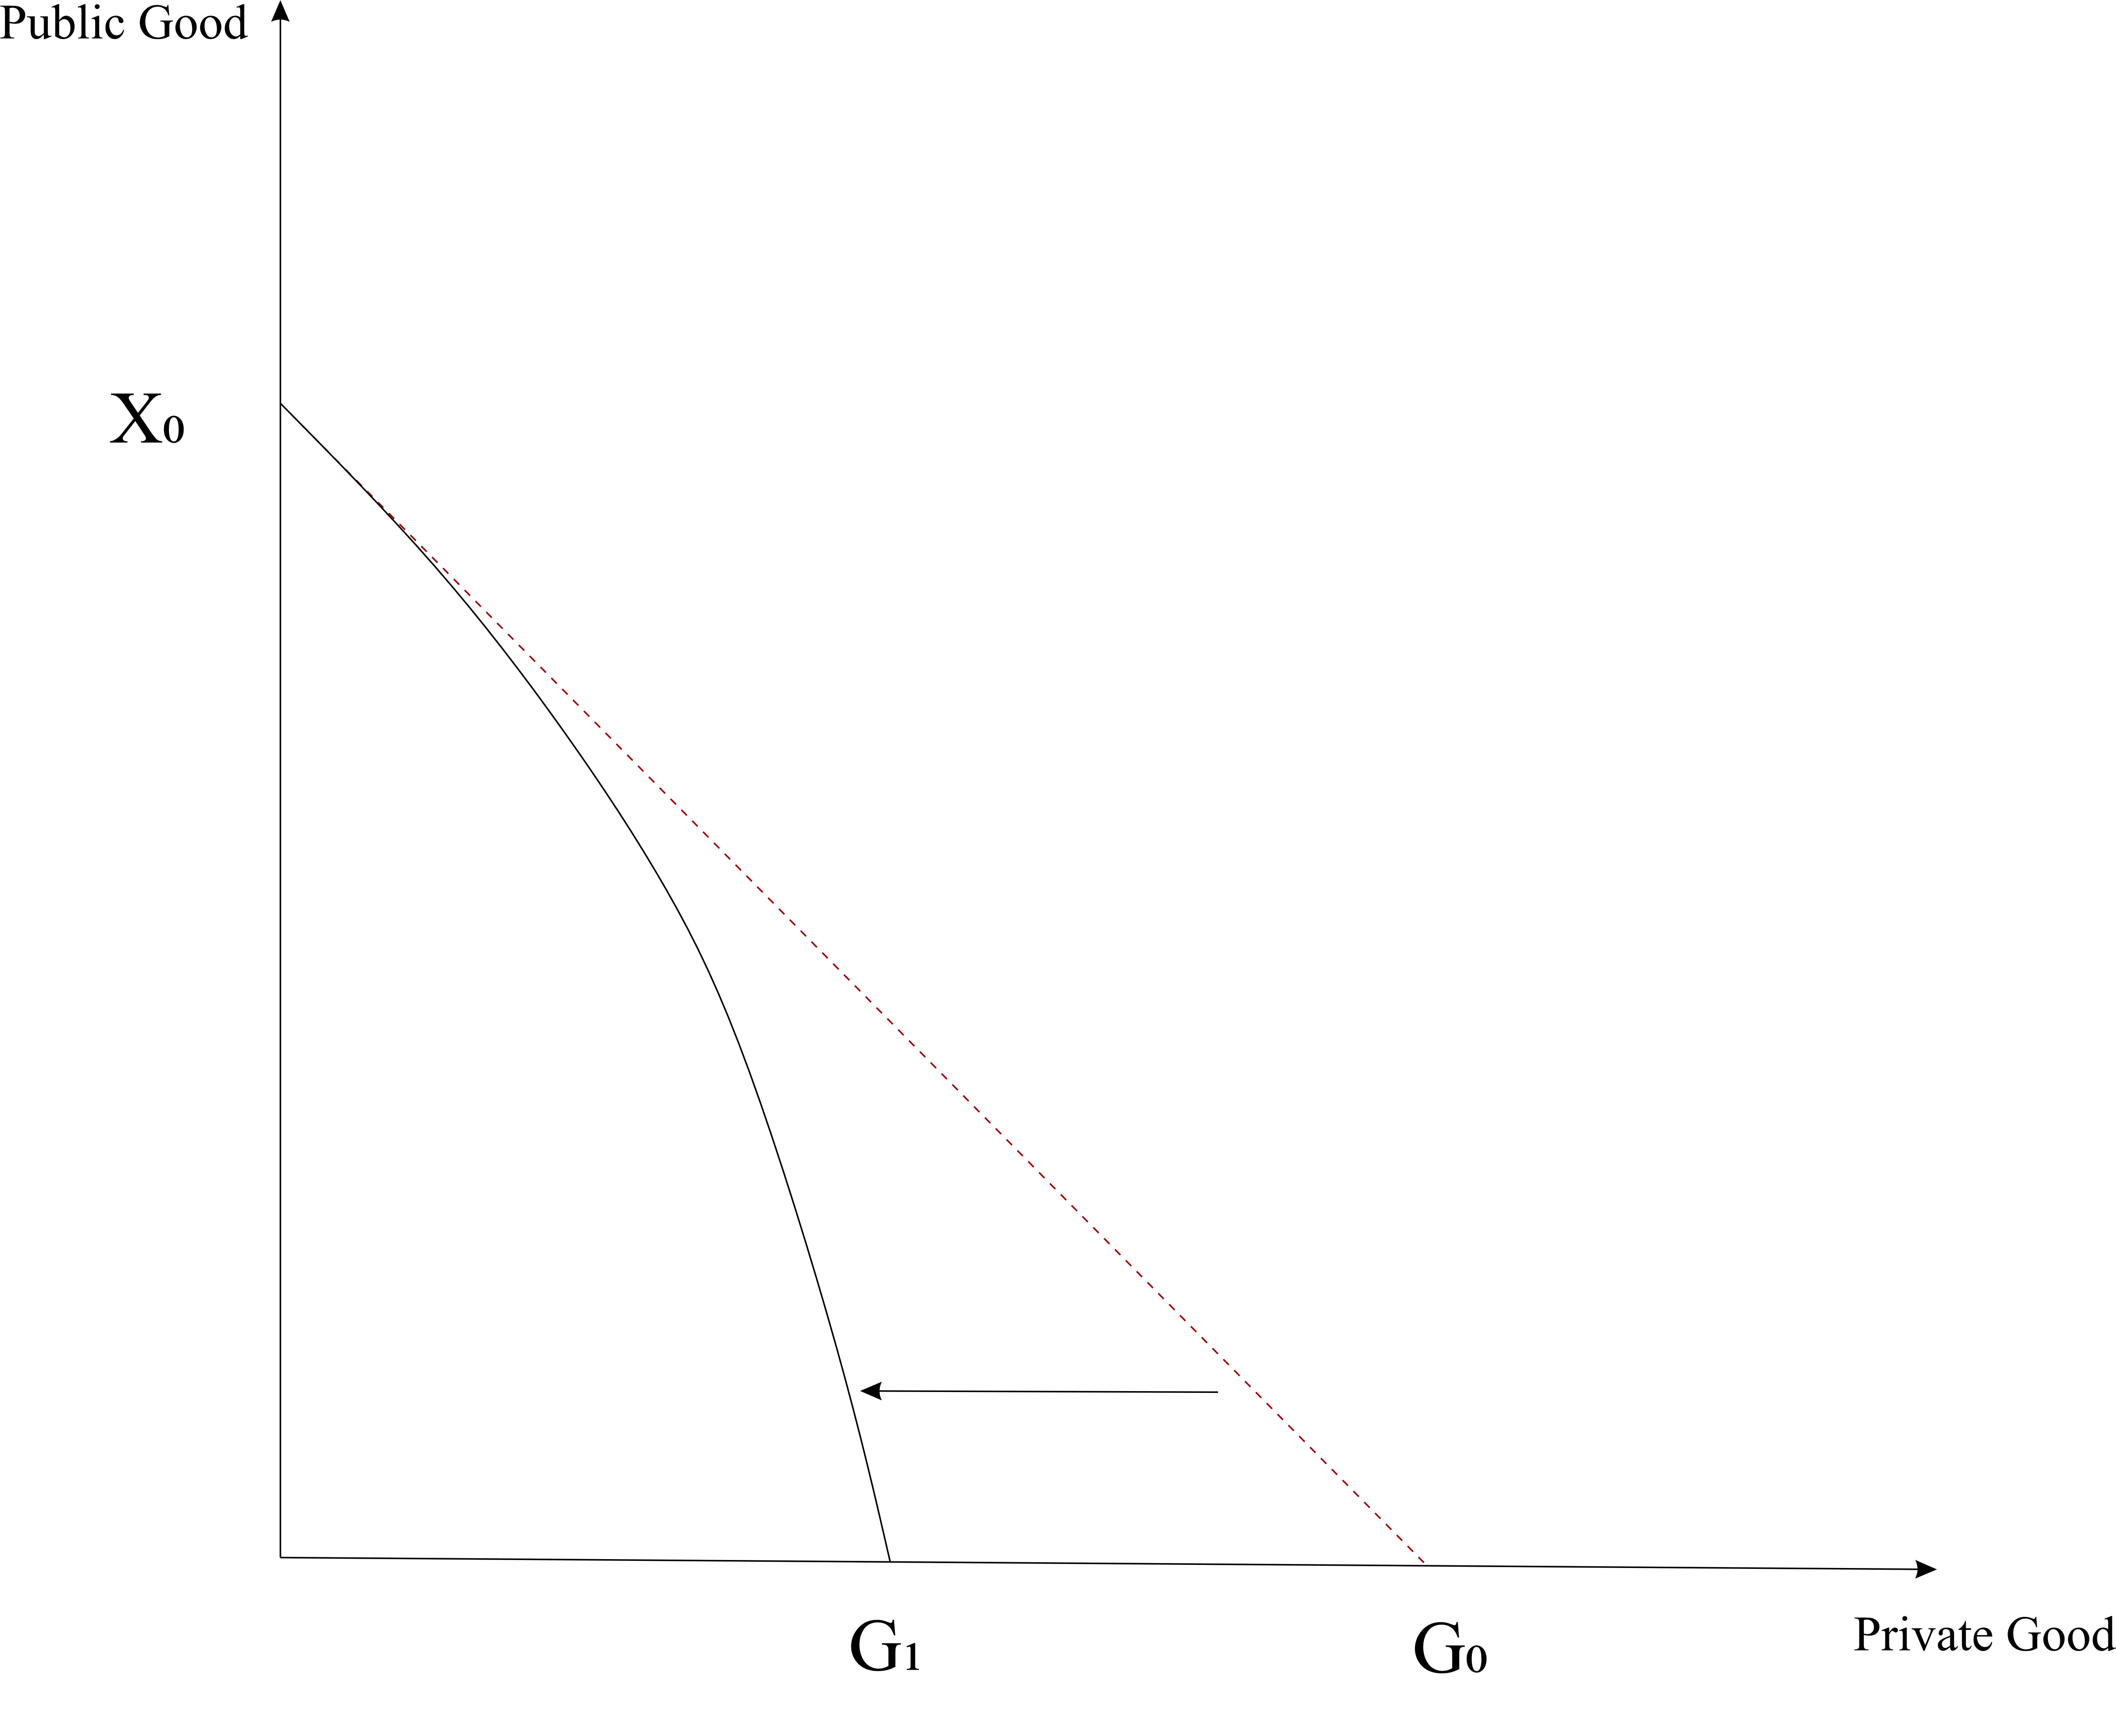
\includegraphics[scale=0.4]{Chapter-4/Figures/budget constrain distortion.jpg}
    \caption[Hamilton's Curved Budget Constraint]{Hamilton's Curved Budget Constrain
        \texttt{} }
    \label{Figure 3.4}
\end{figure}

In reality, the cost of tax collection comes from various sources, including the different levels of administrative ability between federal and state governments. Volden \cite{volden2007intergovernmental} developed a game theory model to simulate the interaction between the federal government and lower-level governments and showed that the different costs of collecting revenue for federal and state governments partially explains the flypaper effect. Dahlby and Ferede \cite{dahlby2016stimulative} argued that the price effect of non-matching grants exists even without fiscal illusion due to subnational governments face information and ability disadvantages, meanwhile Vegh and Vuletin \cite{vegh2016unsticking} came to a similar conclusion. In summary, these researchers suggest that the collection of tax revenue is costly for state and local governments due to factors such as administrative inefficiency and distortion, leading to a preference for using "cheaper" resources such as intergovernmental transfers. Therefore, even non-matching grants or lump-sum grants can have price effects.

Some horizontal government interaction explains this distortion as well, Brueckner \cite{brueckner2003strategic} develops a strategic model to analyze the state and local fiscal behavior, he concludes that the lower-level governments are quite sensitive to other competitors. This sensitivity may explain why state and local government don’t want tax increase revenue to cover the public goods. Other horizontal interaction theory such as yardstick competition or tax competition also explains the sensitivity.

I expand the benchmark model by introducing the distortion of tax collection into it.

\textbf{Ramsey Model with Distortionary Tax Collection}

To capture the distortion effect of the tax,I loosen the 3rd and 5th assumption of the benchmark model. I follow the setting by Carlos and Vuletin \cite{vegh2016unsticking} by adding a taxable private goods $X_t$ to differentiate with the non-taxable private goods $X_{nt}$ and capture the distortion effect of proportional tax. In reality, $X_{nt}$ could express any behavior that representative resident take to avoid the taxation, such as more time on leisure or
The assumption on taxation and representative resident's spending behavior are:
\begin{enumerate}
    \item Three kinds of goods in the economy which are public good $G$ and taxable private good $X_t$ and non-taxable private good $X_{nt}$.\label{Xt}
    \item Resident spend all there income $y$, which is given, on either taxable private goods $X_t$, non-taxable private goods $X_{nt}$ or tax.
    \item The tax is proportionary tax on $X_{t}$, with tax rate $\theta$.
\end{enumerate}

So the budget constrain for resident, local government and the whole economy could be separately list as:
\begin{equation} \label{distortionrct}
    y=X_t(1+\theta)+X_{n t}
\end{equation}
\begin{equation} \label{distortiongct}
    f+\theta X_t=G
\end{equation}
\begin{equation} \label{distortionect}
    y+f=x_t+x_{nt}+G
\end{equation}

Different from Carlos' setting who accept a more general setting on residents' and governments' utility, I set Cobb-Douglas form on utility to get a arithmetic solution. Unlike the benchmark model in Carlos' research, in which he set the linear utility, the Cobb-Douglas setting means the imperfect substitute between private and public goods, which is a more reasonable setting. The distribution on $X_t$, $X_{nt}$ and $G$ should maximize representative resident's utility and government's utility.
\begin{equation} \label{rclgutility}
    \left\{\begin{array}{l}U=A X^\alpha G^{1-\alpha} \\ X=B X_t^\beta X_{n t}^{1-\beta}\end{array}\right.
\end{equation}
Where X represent a composite private good.
For resident, they need to decide $X_t, X_{nt}$ to maximize $U$ subject to equation \ref{distortionrct}. For local government, the problem is to decide the distribute of $X$ and $G$ to maximize $U$, thus the Ramsey problem is to maximize both resident and local governments' utility, which is listed as equation \ref*{rclgutility} subject to equation \ref{distortionrct} and \ref{distortiongct}. For resident, the first order conditions on $X_t, X_{nt}, \lambda_{rc}$ can be listed as:
\begin{align}
    \begin{split}
        \frac{\partial U}{\partial X} \frac{\partial X}{\partial X_t}=(1+\theta) \lambda_{r c} \label{focxt}
    \end{split}                     \\
    \begin{split}
        \frac{\partial U}{\partial X} \frac{\partial X}{\partial X_{nt}}=\lambda_{r c} \label{focxnt}
    \end{split} \\
    \begin{split}
        y=X_t(1+\theta)+X_{nt} \label{foclabrc}
    \end{split}
\end{align}
Solving equation \ref{focxt}, \ref{focxnt} will generate the relationship between $X_t$ and $X_{nt}$ in equilibrium and the level of $\theta$:
\begin{align}
    \begin{split}
        X_{nt}=\frac{(1-\beta)(1+\theta)}{\beta}X_t \label{xtxnt}
    \end{split} \\
    \begin{split}
        \theta=\frac{\beta X_{n t}}{(1-\beta) X_t}-1 \label{theta}
    \end{split}
\end{align}

For local government and Ramsey Planner, they need to decide $G, X_t, X_{nt}$ subject to equation \ref*{distortiongct} and \ref*{distortionect}, the FOCs on $X_t, X_{nt}, G, \lambda_e, \lambda_{lg}$ are:
\begin{align}
    \begin{split}
        \frac{\partial U}{\partial X} \frac{\partial X}{\partial X_t}=\lambda_e+\lambda_{l g}
    \end{split}                                                      \\
    \begin{split}
        \frac{\partial U}{\partial X} \frac{\partial X}{\partial X_{nt}}=\lambda_e +\frac{\beta}{1-\beta} \lambda_{l g}
    \end{split} \\
    \begin{split}
        \frac{\partial U}{\partial G}=\lambda_e+\lambda_{l g}
    \end{split}                                                                                      \\
    \begin{split}
        y+f=x_t+x_{nt}+G
    \end{split}                                                                                                                           \\
    \begin{split}
        f+\theta X_t=G
    \end{split}
\end{align}

Solving equation 3.29 to equation 3.33, I can get the arithmetic solution of $X_t, X_{nt}, G$ as:

\begin{align}
    \begin{split}
        x_t=\frac{\beta y+f}{\alpha \beta+1-\alpha} \cdot \alpha \beta
    \end{split} \\
    \begin{split}
        G=\frac{(\beta y+f)(1-\alpha)}{\alpha \beta+1-\alpha}
    \end{split}
\end{align}

Follow the definition of $fe$ in benchmark model , the flypaper effect under distortionary taxation can be calculated as:

\begin{align}
    \begin{split}
        \frac{d G}{d f}-\frac{d G}{d y}=\frac{(1-\alpha)(1-\beta)}{\alpha \beta+1-\alpha}  \label{feunderdistortion}
    \end{split}
\end{align}
The size of flypaper effect under distortion can be expressed as Figure 3.5. As is shown, the value of flypaper effect is always positive.
\begin{figure}[htbp]
    \centering
    \subfigure[]{
        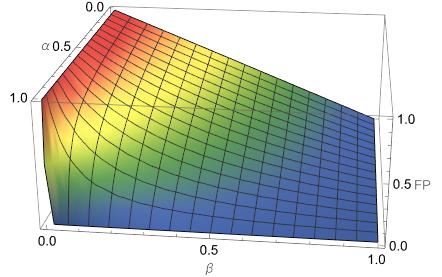
\includegraphics[width=0.45\textwidth]{Chapter-4/Figures/distofp1.jpg}}
    \subfigure[]{
        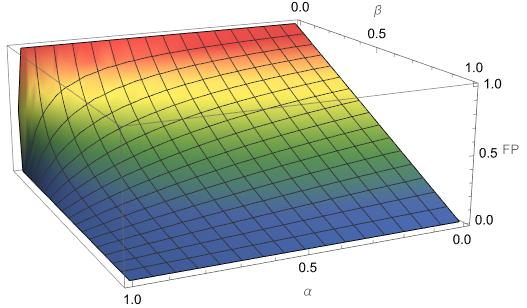
\includegraphics[width=0.45\textwidth]{Chapter-4/Figures/distofp2.jpg}}
    \subfigure[]{
        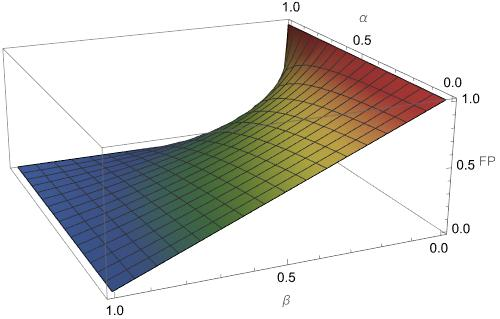
\includegraphics[width=0.45\textwidth]{Chapter-4/Figures/distofp3.jpg}}
    \subfigure[]{
        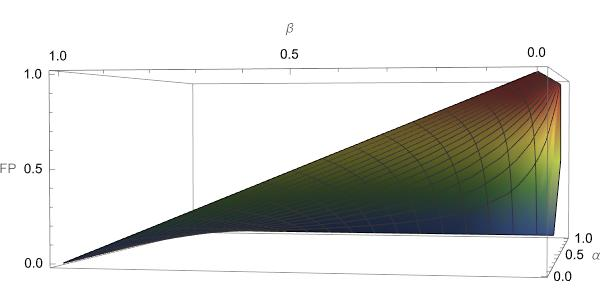
\includegraphics[width=0.45\textwidth]{Chapter-4/Figures/distofp4.jpg}}
    \caption{3-Dimensions Plot of the Fluctuation of Flypaper Effect under Distortion}
    \label{figfeunderdistortion}
\end{figure}

\subsection{Effect of IGT on Local Governments' Spending Segments}
% The investigation on the spending preference is related with the investigation of local governments' tax effort.

Compared to investigations on overall spending amounts, the understanding of the impact of intergovernmental transfers on micro-segmented spending varies. Scholars focus not only on the effect of matching mechanism but also on the effect of purpose restrictions when analyzing the impact of IGT on spending preferences. Specifically, general transfers, such as general revenue sharing in Table \ref{Table 1.1}, and transfers with special purposes, such as block grants and project categorical grants in Table \ref{Table 1.1}, may have different effects on local governments' spending preferences. Some empirical evidence still implies the flypaper effect, meaning that intergovernmental transfers stimulate local governments' spending in specific areas. Feldstein observed that categorical grants in the education field from the Massachusetts state government to local governments lead to higher local government spending on education \cite{feldstein1975wealth}. Karnik and Lalvani \cite{karnik2008flypaper} incorporated the spatial effect into their model when analyzing data from Maharashtra in India. They found that an increase in intergovernmental grants results in urban local governments spending more on specific expenditure categories than they would have with an equivalent increase in incomes.

Another widely discussed phenomenon related to categorical government spending preference is fungibility \cite{pack1993foreign}. Fungibility refers to the fact that intergovernmental transfers received by local governments may substitute their own revenue, which can result in changes to the spending structure based on local government preference, rather than being tied to the strings attached to the intergovernmental transfer. Evidence of this phenomenon can be seen in Latin America, where subnational governments have been found to prefer using transfer funds to cover administrative expenses \cite{stein1999fiscal}. Similarly, research in China has shown that local governments crowd out revenue that should have been invested in public services and instead direct it to productive spending once they receive intergovernmental transfers, even if these transfers are restricted to specific categories \cite{yinheng2011,fuyong2010}.

One potential issue with the investigation of spending preference is that most studies focus solely on individual spending sectors, represented by the lower left quadrant in Figure \ref{Figure 3.1}. However, it is important to recognize that spending preferences cannot be studied in isolation. Therefore, in this study, I will incorporate revenue behavior into the model to provide a more comprehensive evaluation of spending behavior in Section 3.2.

Furthermore, many of the aforementioned investigations rely solely on empirical evidence and lack a general theoretical framework to explain their findings. To address this issue, I will introduce an asymmetric setting into the model and use it to explain spending preferences based on the theoretical framework that I have developed to explain the flypaper effect.



